\begin{frame}
	\frametitle{Taxa Marginal de Substitui\c c\~ao}
	\begin{itemize}
		\item<1-> \'E a taxa \`a qual o consumidor est\'a disposto a trocar um bem pelo outro e ficar indiferente.
		\item<2-> Define-se como a quantidade do bem $Y$ de que est\'a disposto a prescindir, para ter mais uma unidade do bem $X$ e ficar indiferente.
	\end{itemize}
\end{frame}

\begin{frame}
	\frametitle{Taxa Marginal de Subsitui\c c\~ao}
	\begin{center}
		\def\a{1/2}
		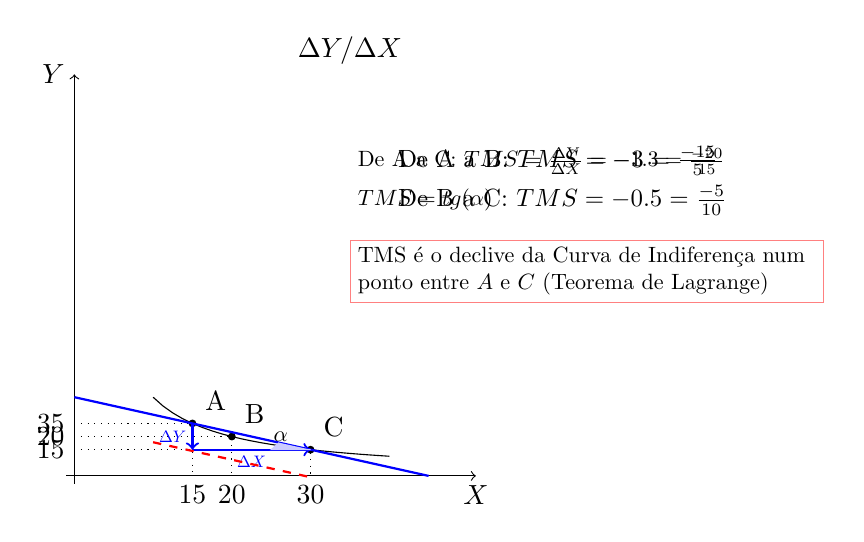
\begin{tikzpicture}[
			scale = 1,
			declare function = {i(\x) = (1/(\x^\a))^(1/(1-\a));},
			declare function = {di(\x) = -(\a/(1-\a))*(1/(\x^(1/(1-\a))));},
			declare function = {tang(\x) = i(1.5) - (i(3)-i(1.5)) + ((i(3)-i(1.5))/(3-1.5)) * \x;},
			declare function = {tg(\x) = tang(\x) - 0.35;}
		]

		\draw[->] (0,-0.1) -- (0,5.1) node[left]{$Y$};
		\draw[->] (-0.1,0) -- (5.1,0) node[below]{$X$};

		\draw(3.5,5.1) node[above] {$\Delta Y/\Delta X$};

		\draw[domain=1:4,variable=\x] plot (\x,{i(\x)});

		\draw[dotted] (0,{i(1.5)}) node[left] {35} -- (1.5,{i(1.5)}) node[circle,fill,inner sep=1pt,label = above right:A]{} -- (1.5,0)node[below] {15};
		\draw[dotted] (0,{i(3)}) node[left] {15} -- (3,{i(3)}) node[circle,fill,inner sep=1pt,label = above right:C]{} -- (3,0)node[below] {30};

		\only<1>{
			\draw[dotted] (0,{i(2)}) node[left] {20} -- (2,{i(2)}) node[circle,fill,inner sep=1pt,label = above right:B]{} -- (2,0)node[below] {20};
			\draw(4,4) node[right,text width = 0.5\textwidth, scale = 0.9] {De A a B: $TMS = -3 = \frac{-15}{5}$};
			\draw(4,3.5) node[right,text width = 0.5\textwidth, scale = 0.9] {De B a C: $TMS = -0.5 = \frac{-5}{10}$};
		}

		\onslide<2->{
			\draw(3.5,4) node[right,text width = 0.6\textwidth, scale = 0.8] {De A a C: $TMS = \frac{\Delta Y}{\Delta X} = -1.3 = \frac{-20}{15}$};
			\draw[blue,thick,domain=0:(-(2*i(1.5)-i(3))*(3-1.5)/(i(3)-i(1.5))),variable=\x] plot (\x,{tang(\x)});
		}
		
		\onslide<3->{
			\draw[blue,thick,->] (1.5,{tang(1.5)}) -- (1.5,{tang(3)}) node [midway, left,scale=0.6] {$\Delta Y$};
		}
		\onslide<4->{
			\draw[blue,thick,->] (1.5,{tang(3)}) -- (3,{tang(3)}) node [midway, below,scale=0.6] {$\Delta X$};
		}
		
		\onslide<5->{
			\draw[red,thick,dashed,domain=1:3,variable=\x] plot (\x,{tg(\x)}); 
		}

		\onslide<6->{
			\draw[fill,blue!20] (3,{i(3)}) node[black,scale=0.8,above left] {$\alpha\ \ $} -- (2.5,{tang(3)}) -- (2.6,{tang(2.6)});
			\draw(3.5,3.5) node[right,text width = 0.6\textwidth, scale = 0.8] {$TMS=tg(\alpha)$};
		}

		\onslide<7->{
			\draw[] (3.5,3) node[below right,rectangle,draw=red!50,scale=0.8,text width=0.6\textwidth] {TMS \'e o declive da Curva de Indiferen\c ca num ponto entre $A$ e $C$ (Teorema de Lagrange)};
		}

		\end{tikzpicture}
	\end{center}
\end{frame}

\begin{frame}
	\frametitle{Taxa Marginal de Substitui\c c\~ao}
	Ao longo da curva de indiferen\c ca apresentada (convexa), a TMS \'e decrescente em valor absoluto:
	\vspace{0.2cm}
	\begin{itemize}
		\item<2-> Admitimos que o consumidor valoriza mais o bem de que disp\~oe em menor quantidade
		\item<3-> Quanto maior a quantidade de um bem de que o consumidor disp\~oe, menor o valor que atribui a uma unidade adicional, porque fica mais perto do ponto de saciedade, onde o consumo adicional deixa de ser desej\'avel!
	\end{itemize}
\end{frame}

\begin{frame}
	\frametitle{Axiom\'atica de Prefer\^encias (cont.)}
	\begin{enumerate}
		\item<2->Desejabilidade $\Rightarrow$ as curvas de indiferen\c ca t\^em inclina\c c\~ao negativa!
		\item<3->As prefer\^encias s\~ao completas: dados dois cabazes, o consumidor sabe sempre dizer qual a rela\c c\~ao de prefer\^encias entre eles $\Rightarrow$ todos os cabazes pertencem a uma curva de indiferen\c ca!
		\begin{itemize}
			\item<4-> Quanto mais alta for a curva onde se localiza um cabaz, maior a satisfa\c c\~ao que resulta do consumo desse cabaz (desejabilidade...)
		\end{itemize}
	\end{enumerate}
\end{frame}

\begin{frame}
	\frametitle{Curvas de Indiferen\c ca ``bem comportadas''}
	\begin{center}
		\def\a{1/2}
		\begin{tikzpicture}[
			scale = 1,
			declare function = {i(\x,\u) = (\u/(\x^\a))^(1/(1-\a));}
		]

		\draw[->] (0,-0.1) -- (0,5.1) node[left]{$Y$};
		\draw[->] (-0.1,0) -- (5.1,0) node[below]{$X$};

		\draw[samples=100,domain=0.9:5,variable=\x] plot (\x,{i(\x,1)});

		\draw (2,{i(2,1)}) node[circle,fill,inner sep=1pt,label = above right:A]{};
		\draw (1.1,{i(1.1,1)}) node[circle,fill,inner sep=1pt,label = above right:B]{};

		\draw (2.2,{i(2.2,2)}) node[circle,fill,inner sep=1pt,label = above right:C]{};
		\draw (3,{i(3,2)}) node[circle,fill,inner sep=1pt,label = above right:D]{};

		\draw (2.6,{i(2.6,3)}) node[circle,fill,inner sep=1pt,label = above right:E]{};
		\draw (3.2,{i(3.2,3)}) node[circle,fill,inner sep=1pt,label = above right:F]{};

		\draw (1.2,{i(1.2,0.6)}) node[circle,fill,inner sep=1pt,label = above right:G]{};
		
		\onslide<2->{
			\draw [samples=100,blue,domain=1.8:5,variable=\x] plot (\x,{i(\x,2)});
			\draw [samples=100,blue,domain=2.5:5,smooth,variable=\x] plot (\x,{i(\x,3)});
			\draw [samples=100,red,domain=0.6:5,variable=\x] plot (\x,{i(\x,0.6)});
		}

		\only<3-4>{
			\draw[] (4.5,5) node[above right,scale=0.7] {$\sim$ Significa ``indiferente a''};
			\draw[] (4.5,4.5) node[above right,scale=0.7] {$\succ$ Significa ``preferido a''};

		}

		\only<4>{
			\draw[] (4.5,4) node[above right, scale=0.7] {$E\sim F\succ C\sim D \succ B \sim A \succ G$};
			\draw[->,thick,green] (1,1) -- (4,4) node [green!80!black,below right,scale=0.8] {Sentido de aumento da satisfa\c c\~ao};
		}
		\end{tikzpicture}
	\end{center}
\end{frame}

\begin{frame}
	\frametitle{Axiom\'atica de Prefer\^encias (cont.)}
	\begin{enumerate}
		\item<1-> Desejabilidade
		\item<2-> As prefer\^encias s\~ao completas
		\item<3-> As prefer\^encias s\~ao transitivas:
	\end{enumerate}
	\onslide<3->{Se:
	\begin{center}
		A \'e preferido a B\\
		B \'e preferido a C\\
		Ent\~ao A \'e preferido a C!
	\end{center}
	}
\end{frame}

\begin{frame}
	\frametitle{As curvas de Indiferen\c ca n\~ao se podem cruzar}
	\begin{columns}
		\begin{column}{0.47\textwidth}
			\begin{center}
				\def\a{1/2}
				\def\inter{1.365}
				\begin{tikzpicture}[
						scale = 0.7,
						every node/.style = {scale = 0.7},
						declare function = {i(\x,\u) = (\u/(\x^\a))^(1/(1-\a));}
					]

					\draw[->] (0,-0.1) -- (0,5.1) node[left]{$Y$};
					\draw[->] (-0.1,0) -- (5.1,0) node[below]{$X$};

					\draw[domain=0.9:5,variable=\x] plot (\x,{i(\x,1)});
					\draw[domain=0.5:4.5,variable=\x] plot (\x,{i(\x+0.5,1)+1});

					\draw (2,{i(2,1)}) node[circle,fill,inner sep=1.5pt,label = above right:A]{};
					\draw (1.1,{i(1.1,1)}) node[circle,fill,inner sep=1.5pt,label = above right:B]{};

					\draw (\inter,{i(\inter,1)}) node[circle,fill,inner sep=1.5pt,label = above right:C]{};
					\draw (2.2,{i(2.7,1)+1}) node[circle,fill,inner sep=1.5pt,label=above right:D]{};
					
			\end{tikzpicture}
			\end{center}
		\end{column}
		\begin{column}{0.47\textwidth}
			\begin{itemize}
				\item Estas curvas de indiferen\c ca n\~ao refleitem prefer\^encias transitivas.
				\item<2-> $D\succ A$
				\item<3-> Pero $D\sim C$,
				\item<4-> E $C\sim A$!!!
			\end{itemize}
		\end{column}
	\end{columns}
\end{frame}

\begin{frame}
	\frametitle{Racionalidade}
	\begin{itemize}
		\item<1-> Em contexto de desejabilidade (n\~ao saciedade), as prefer\^encias dizem-se racionais, se forem completas e transitivas.
		\item<2-> Outras hip\'oteses necess\'arias na Teoria do Consumidor:
		\begin{itemize}
			\item<3-> Informa\c c\~ao completa
			\item<4-> Continuidade do espa\c co or\c camental
			\item<5-> Independ\^encia das escolhas entre consumidores
		\end{itemize}
	\end{itemize}
\end{frame}


\begin{frame}
	\frametitle{Fun\c c\~ao Utilidade}
	A fun\c c\~ao de utilidade \'e uma representa\c c\~ao num\'erica da rela\c c\~ao de prefer\^encia, que transforma cabazes de consumo num valor (utilidade) e \'e tal que dados dois cabazes $A$ e $B$:
	\begin{align*}
		U(A) &> U(B) \quad \Leftrightarrow \quad \text{A \'e preferido a B}\\
		U(A) &= U(B) \quad \Leftrightarrow \quad \text{A \'e indiferente a B}
	\end{align*}
\end{frame}


\begin{frame}
	\frametitle{Fun\c c\~ao Utilidade}
	A fun\c c\~ao de utilidade \'e apenas uma \textbf{\underline{rela\c c\~ao ordinal}}, resultando numa ordena\c c\~ao de cabazes, atribuindo um valor maior aos cabazes preferidos. \textbf{\underline{Esse valor, por si s\'o, n\~ao tem significado cardinal.!}}\pause

	\vspace{0.2cm}

	\underline{Consequ\^encia:} h\'a muitas fun\c c\~oes utilidade que expressam as mesmas prefer\^encias, basta que preservem a ordena\c c\~ao dos cabazes...
\end{frame}

\begin{frame}
	\frametitle{Fun\c c\~ao Utilidade}
	Ex. $A(20,20)$ \'e preferido a $B(10,10)$. Esta rela\c c\~ao pode ser descrita por qualquer uma das fun\c c\~oes seguintes:
	\begin{align*}
		U(x,y) &= x^{0.5}y^{0.5}\\
		U(x,y) &= 10x^{0.5}y^{0.5}\\
		U(x,y) &= 0.5(ln(x)+ln(y))\\
		U(x,y) &= 223.2(ln(x)+ln(y))
	\end{align*}
\end{frame}


\begin{frame}
	\frametitle{Fun\c c\~ao Utilidade}
	Se uma fun\c c\~ao utilidade $U(x,y)$ representar uma ordem de prefer\^encias, qualquer curva de indeferen\c ca \'e constitu\'ida por todos os cabazes que est\~ao associados \`a mesma utilidade:
	\begin{align*}
		\forall(x,y)&:U(x,y)=\overline{U}\\
		&\text{ou}\\
		\forall(x,y)&:\Delta U = 0
	\end{align*}
\end{frame}

\begin{frame}
	\frametitle{Escolha \'Optima}
	\'E o ponto de escolha tal que o consumidor atinge o m\'aximo de utilidade poss\'ivel (localiza-se na curva de indiferen\c ca o mais alta poss\'ivel), dado que n\~ao pode ultrapassar o or\c camento dispon\'ivel para consumo.
\end{frame}

\begin{frame}
	\frametitle{Escolha do consumidor}
	\begin{center}
		\def\a{0.5}
		\def\u{1.55}
		\def\d{0.5}
		\def\w{10}
		\def\px{3}
		\def\py{3.5}
		\begin{tikzpicture}[
			scale = 1,
			every node/.style={scale = 1},
			declare function = {ic(\x,\u) = ((\u)/(\x^\a))^(1/(1-\a));},
			declare function = {bc(\x,\w) = \w/\py - (\px/\py)*\x;}
			]

			\draw[->] (-0.1,0) -- (5.1,0)node[below right] {$X$};
			\draw[->] (0,-0.1) -- (0,5.1)node[above left] {$Y$};

			\draw[] (4,4) node[right,scale=0.6] {$A^{*}(P,W):Max_{x,y} U(x,y)\wedge Xp_x+Yp_y=W$};

			\onslide<2->{\draw[samples=100,blue,domain=0:(\w/\px),variable=\x] plot (\x,{bc(\x,\w)});}
			\onslide<3-4>{\draw[samples=100,red,domain=1:5,variable=\x] plot (\x,{ic(\x,\u+\d)});}
			\only<4>{\draw[samples=100,red,domain=.3:5,variable=\x] plot (\x,{ic(\x,\u-\d)});}
			\onslide<5->{
				\draw[samples=100,red,domain=.6:5,variable=\x] plot (\x,{ic(\x,\u)});
				\draw(1.65,{ic(1.65,\u)}) node[red,circle,fill,inner sep=1.5pt]{};
				\draw[dashed](1.65,0) node[below]{$x^*$} -- (1.65,{ic(1.65,\u)}) -- (0,{ic(1.65,\u)}) node [left]{$y^*$};
			}
 
		\end{tikzpicture}
	\end{center}
\end{frame}